\chapter{Language of Category Theory}
\section{Universe}
\begin{definitionenv}
    We call \textbf{universe} any set $\mathcal{U}$ whose elements are sets, satisfying the following conditions:
    \begin{enumerate}[label=(\alph*)]
        \item $\varnothing \in \mathcal{U}$.
        \item If $A\in \mathcal{U}$ and $B\in A$, then $B\in \mathcal{U}$.
        \item If $A\in \mathcal{U}$, then $\mathscr{P}(A)\in \mathcal{U}$.
        \item If $I\in \mathcal{U}$ and $(A_i)_{i\in I}\in \mathcal{U}^{I}$, then $$\bigcup_{i\in I} A_i\in \mathcal{U}.$$
    \end{enumerate}
\end{definitionenv}
\begin{axiomenv}
Every set belongs to some universe.
\end{axiomenv}
\begin{propositionenv}
    Let $\mathcal{U}$ be a universe
    \begin{enumerate}[label=(\arabic*)]
        \item If $A\in \mathcal{U}$ and $B\subseteq A$, then $B\in \mathcal{U}$.
        \item For any $A\in \mathcal{U}$, one has $\{A\}\in \mathcal{U}$.
        \item If $A,B\in \mathcal{U}$, then $\{A,B\}\in \mathcal{U}$.
        \item If $A,B\in \mathcal{U}$, then $(A,B)\in \mathcal{U}$, where $$ (A,B)\coloneq \{\{A\},\{A,B\}\}.$$
        \item If $X,Y\in \mathcal{U}$, then the Cartesian product $X\times Y\in \mathcal{U}$, where $$ X\times Y\coloneq \{(x,y)\mid x\in X, y\in Y\}.$$
        \item If $X,Y\in \mathcal{U}$, then the set of all correspondences from $X$ to $Y$ belongs to $\mathcal{U}$.
        \item If $X,Y\in \mathcal{U}$, then $Y^X\in \mathcal{U}$.
        \item Let $I\in \mathcal{U}$, $(X_i)_{i\in I}\in \mathcal{U}^I$, then $$\prod_{i\in I} X_i \in \mathcal{U}.$$
    \end{enumerate}
\end{propositionenv}
\begin{proofenv}
\quad
\begin{enumerate}[label=(\arabic*)]
    \item By (c), $\mathscr{P}(A)\in \mathcal{U}$ and as $B\in \mathscr{P}(A)$ then from (b), we get $B\in \mathcal{U}$.
    \item By (c), $\mathscr{P}(A)\in \mathcal{U}$, as $\{A\}\subseteq \mathscr{P}(A)$ one can deduce from (1) $\{A\}\in \mathcal{U}$.
    \item By (c) and (a) $$\mathscr{P}(\mathscr{P}(\varnothing))=\{\varnothing,\{\varnothing\}\}\in \mathcal{U}.$$ $A,B\in \mathcal{U}$ then by (2), $\{A\},\{B\}\in \mathcal{U}$, by (d), $\{A,B\}=\{A\}\cup\{B\}\in \mathcal{U}.$
    \item By (2), $\{A\}\in \mathcal{U}$, by (3) $\{A,B\}\in \mathcal{U}$ and again by (3), $\{\{A\},\{A,B\}\}\in \mathcal{U}$.
    \item $X,Y\in\mathcal{U}$, so for $x\in X$, $y\in Y$, by (b), $x,y\in U$. By (4), $(x,y)\in \mathcal{U}$, by (2), $\{(x,y)\}\in \mathcal{U}$ and therefore $$\{x\}\times Y = \bigcup_{y\in Y} \{(x,y)\}\in \mathcal{U}.$$ Still by (2), $\dis X\times Y = \bigcup_{x\in X}\{x\}\times Y\in \mathcal{U}$.
    \item A correspondence from $X$ to $Y$ is of the form $f = ((X,Y), \Gamma)$, where $\Gamma \subseteq X\times Y$. By (5) and (c) and (b) $\Gamma \in \mathcal{U}$. By (4), $f \in \mathcal{U}$, and by (2) $\{(X,Y),\Gamma\}\in \mathcal{U}.$ Finally, by (d) $$\bigcup_{\Gamma \in \mathscr{P}(X\times Y)}\{((X,Y),\Gamma)\} \in \mathcal{U}.$$
    \item $Y^X$ is a subset of the set of correspondences from $X$ to $Y$, so by (1) and (b), $Y^X\in \mathcal{U}$.
    \item Let $\dis X=\bigcup_{i\in I}X_i \in \mathcal{U}$, note that $\dis \prod_{i\in I}X_i \subseteq X^I.$ So by (1) and (7), $\dis \prod_{i\in I}X_i \in \mathcal{U}$.
\end{enumerate}
\end{proofenv}
\begin{remark}
    All we have mentioned are sets. And here the ordered pair $(A,B)$ is given by $(A,B)=\{\{A\},\{A,B\}\}$, we can regard it as a kind of coding method, then we can also regard the tuple $(A,B)$ as a set. This makes the problem easy to discuss.
\end{remark}
\section{Category}
\begin{definitionenv}
    Let $\mathcal{U}$ be a universe. We call $\mathcal{U}$-category $\mathcal{C}$ the data consist of
    \begin{enumerate}[label=(\roman*)]
        \item A set $\Obj(\mathcal{C})$. (The elements of which are called objects.)
        \item For any $(X,Y) \in \Obj(\mathcal{C})\times \Obj(\mathcal{C})$ a set $\mathcal{C}(X,Y)\in \mathcal{U}$. (The elements of which are called morphisms from $X$ to $Y$.)
        \item For any $(X,Y,Z)\in \Obj(\mathcal{C})^3$, we have a composition mapping
$$
            \begin{array}{rcl}
            \mathcal{C}(X,Y)\times \mathcal{C}(Y,Z) &\rightarrow &\mathcal{C}(X,Z)\\ 
            (f,g)&\mapsto & g\circ f
            \end{array}
$$
            satisfying the following axioms:
            \begin{enumerate}[label=(\alph*)]
                \item For any $X\in \Obj(\mathcal{C})$, there exists $\mathrm{Id}_X\in \mathcal{C}(X\times X)$ (called the identity morphism of $X$) such that $Y\in \Obj(\mathcal{C})$, one has
                $$\forall f\in \mathcal{C}(X,Y), f\circ \mathrm{Id}_X = f\ ,\forall g\in \mathcal{C}(Y,X), \mathrm{Id}_X\circ g = g$$
                \item For any $(X,Y,Z,W)\in \Obj(\mathcal{C})^4$, $f\in \mathcal{C}(X,Y)$, $g\in \mathcal{C}(Y,Z)$, $h\in \mathcal{C}(Z,W)$, one has $$ h\circ(g\circ f) = (h\circ g)\circ f.$$
                    If $\Obj(\mathcal{C})\in \mathcal{U}$, then we say that $\mathcal{C}$ is \textbf{$\mathcal{U}$-small}. If $\Obj(\mathcal{C})$ is finite and $\mathcal{C}(X,Y)$ is finite for any $X,Y\in \Obj(\mathcal{C})$, then we say that $\mathcal{C}$ is a \textbf{finite category}.
            \end{enumerate}
    \end{enumerate}
\end{definitionenv}
\begin{exampleenv}
    Let $\mathcal{U}$ be a universe. The elements of $\mathcal{U}$ are sets (by definition). Together with (standard set-theoretic) mappings as morphisms, they form a category denoted by $\mathcal{U}$-set. The objects of $\mathcal{U}$-set are the elements of $\mathcal{U}$ and for any $A,B\in \mathcal{U}$,
    $$ \mathcal{U}\text{-}\mathrm{set}(A,B)$$
    is just the set of all mappings from $A$ to $B$.
\end{exampleenv}
\begin{remark}
    In practice, we often omit the mention of the universe $\mathcal{U}$ in which we consider the category theory. With this abbreviation, a $\mathcal{U}$-category is simply called a category. A $\mathcal{U}$-small category is called a small category. Similarly $\mathcal{U}$-set is typically denoted by set.
\end{remark}
\begin{notationenv}[also example]
    \quad
\begin{enumerate}[label=(\arabic*)]
    \item $\mathbf{Top} = \{\text{topological spaces with continuous mappings between them}\}$
    \item $\mathbf{Gp} = \{\text{groups, homomorphisms of monoids}\}$
    
        $\mathbf{Mon} = \{\text{monoid, homomorphism of monoids}\}$

        $\mathbf{Ab}= \{\text{abelian groups, homomorphisms of groups}\}$
    \item $\mathbf{Ring} = \{\text{Unitary rings, homomorphisms of unitary rings}\}$
    \item $\mathbf{K}\text{-}\mathbf{Mod} = \{\text{left-K-modules, }\mathrm{Hom}_K(M,N)\}$, where $K$ is a unitary ring and $M,N$ left $K$-modules.
    \item $\mathbf{Alg}_K=\{K\text{-algebras, homomorphisms of }K\text{ algebras}\}$, where $K$ is a commutative unitary ring.
        Also, $\mathbf{CAlg}$ for those commutative.
\end{enumerate}
\end{notationenv}
\begin{remark}
    Let $K$ be a commutative unitary ring. Recall that a $K$-algebra is a $K$-module $A$ together with a bilinear mapping $$A\times A\rightarrow A$$ such that $A$ equipped with this bilinear mapping forms a unitary ring.
\end{remark}
\begin{notationenv}
    Let $\mathcal{C}$ be a category, $X,Y\in \Obj(\mathcal{C})$. We often write 
    $$ f: X\rightarrow Y \text{ or } X\overset{f}{\longrightarrow} Y$$
    to denote $f\in \mathcal{C}(X,Y)$.
\end{notationenv}
\begin{propositionenv}
    Let $\mathcal{C}$ be a category, $X\in \Obj(\mathcal{C})$. The identity morphism of $X$ is unique.
\end{propositionenv}
\begin{proofenv}
    $ \Id_X = \Id_X \circ \Id_X' = \Id_X'.$
\end{proofenv}
\begin{definitionenv}
    Let $\mathcal{C}$ be a category and $f:X\rightarrow Y$ be a morphism. We say that $f$ is left invertible if there exists $g:Y\rightarrow X$ such that $g\circ f=\Id_X$. We say that $f$ is right invertible if there exists $h:Y\rightarrow X$ such that $f\circ h=\Id_Y$.
\end{definitionenv}
\begin{propositionenv}
    Suppose that $f$ is left invertible and right invertible. Then $f$ has only one left inverse and only one inverse, and they are equal.
\end{propositionenv}
\begin{proofenv}
    Let $g$ be a left inverse and $h$ be a right inverse of $f$.
    $$g = g\circ \Id_Y = g\circ \left(f\circ h\right)= \left(g\circ f\right)\circ h = \Id_X\circ h = h.$$
\end{proofenv}
\begin{definitionenv}
    Let $\mathcal{C}$ be a category and $f:X\rightarrow Y$ be a morphism in $\mathcal{C}$. If $f$ is left and right invertible, there exists a unique morphism $f^{-1}:Y\rightarrow X$ such that
    $$f\circ f^{-1}=\Id_{Y}, f^{-1}\circ f=\Id_{X}.$$
    In this case, we say that $f$ is invertible (or is an isomorphism) and $f^{-1}$ is called the inverse of $f$.
\end{definitionenv}
\begin{exampleenv}
    $\Obj(\mathcal{C})=\{*\}$, $\mathcal{C}(*,*)=(M,\cdot)$ a monoid.
    $$\begin{array}{rcl}
        \mathcal{C}(*,*)\times\mathcal{C}(*,*)&\rightarrow&\mathcal{C}(*,*)\\
        (a,b)&\mapsto& ab
    \end{array}$$
    identity morphism $\Id_X$ is given by the neutral element of $M$.
\end{exampleenv}
\begin{propositionenv}
    Let $\mathcal{C}$ be a category. $X\overset{f}{\rightarrow}Y\overset{g}{\rightarrow}Z$ be a morphism of $\mathcal{C}$. If $f$ and $g$ are isomorphism, so is $g\circ f$. Moreover,
    $$\left(g\circ f\right)^{-1} = f^{-1}\circ g^{-1}.$$
\end{propositionenv}
\begin{proofenv}
    $$\left(f^{-1}\circ g^{-1}\right) \circ\left(g\circ f\right) = f^{-1} \circ \left(g^{-1}\circ g\right)\circ f = f^{-1} \circ \Id_{Y} \circ f = f^{-1}\circ f = \Id_{X}.$$
    $$\left(g\circ f\right)^{-1} \circ \left(f^{-1}\circ g^{-1} \right) = g\circ\left(f\circ f^{-1}\right)\circ g^{-1} = g \circ \Id_{Y} \circ g^{-1} = g\circ g^{-1} =\Id_Z.$$
\end{proofenv}
\begin{definitionenv}
    Let $\mathcal{C}$ be a category. We denote by $\mathcal{C}^{\op}$ the following category
    \begin{itemize}
        \item $\Obj(\mathcal{C}^{\op}) = \Obj(\mathcal{C})$.
        \item $\forall (X,Y)\in \Obj(\mathcal{C})^2$, $\mathcal{C}^{\op}(X,Y) = \mathcal{C}(Y,X).$
        \item $$\begin{array}{rcl}
            \mathcal{C}^{\op}(X,Y)\times \mathcal{C}^{\op}(Y,Z)&\rightarrow&\mathcal{C}^{op}(X,Z)\\
            (f,g)&\mapsto&f\circ g.
        \end{array}$$
    \end{itemize}
        \begin{center}
    \begin{tikzcd}
X \arrow[r,  "f"] \arrow[dr,  swap,  "f\circ g"] &\displaystyle Y \arrow[d,  "g"] \\
& Z
\end{tikzcd}
\end{center}
\end{definitionenv}
\begin{definitionenv}
    A diagram of morphism in a category $\mathcal{C}$ is a directed graph whose vertices are objects and arrows are morphisms.

    \quad We say that a diagram is commutative if for any pair of vertices $(X,Y)$, the morphism obtained by composing along different paths linking $X$ to $Y$ are the same.
\end{definitionenv}
\begin{exampleenv}
    \quad \newline
    Commutative if $g\circ f =h$.
    \begin{center}
    \begin{tikzcd}
X \arrow[r,  "f"] \arrow[dr,  swap,  "h"] &\displaystyle Y \arrow[d,  "g"] \\
& Z
\end{tikzcd}
\end{center}
Commutative if $g\circ f =k\circ h$.
    \begin{center}
    \begin{tikzcd}
X \arrow[r,  "f"] \arrow[d,  swap,  "h"] &\displaystyle Y \arrow[d,  "g"] \\
Z \arrow[r,"k"]& W
\end{tikzcd}
\end{center}
\end{exampleenv}
\newpage
\section{Functors}
\begin{definitionenv}
    Let $\mathcal{C}$ and $\mathcal{D}$ be categories. We call \textbf{functor} from $\mathcal{C}$ to $\mathcal{D}$ the following data:
    \begin{enumerate}[label=(\alph*)]
        \item A mapping $$\begin{array}{rcl}
            \Obj(\mathcal{C})&\rightarrow&\Obj(\mathcal{D})\\
            X&\mapsto & F(X).
        \end{array}$$
        \item $\forall(X,Y)$ couple of objects in $\mathcal{C}$, a mapping
        $$\begin{array}{rcl}
            \mathcal{C}(X,Y)&\rightarrow&\mathcal{D}(F(X),F(Y))\\
            f&\mapsto & F(f).
        \end{array}$$
        which satisfy the following axioms
        \begin{enumerate}[label=(\roman*)]
            \item $\forall X\in \Obj(\mathcal{C})$, $F(\Id_X)=\Id_{F(X)}$.
            \item For any morphism $X\overset{f}{\rightarrow}Y\overset{g}{\rightarrow}Z$ in $\mathcal{C}$,
            $$F\left(g\circ f\right) = F(g)\circ F(f).$$
        \end{enumerate}
    \end{enumerate}
    We use the expression $F:\mathcal{C}\rightarrow\mathcal{D}$ to denote a functor from $\mathcal{C}$ to $\mathcal{D}$.
    \begin{center}
        

\tikzset{every picture/.style={line width=0.75pt}} %set default line width to 0.75pt        

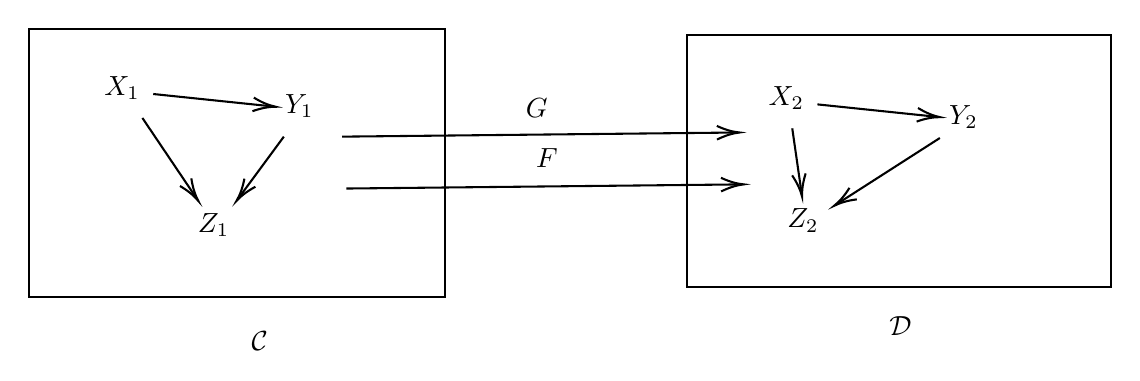
\begin{tikzpicture}[x=0.75pt,y=0.75pt,yscale=-1,xscale=1]
%uncomment if require: \path (0,300); %set diagram left start at 0, and has height of 300

%Shape: Rectangle [id:dp583091700239915] 
\draw   (66,78) -- (266.5,78) -- (266.5,207.07) -- (66,207.07) -- cycle ;
%Shape: Rectangle [id:dp2047555694997948] 
\draw   (383,81) -- (587.5,81) -- (587.5,202.33) -- (383,202.33) -- cycle ;
%Straight Lines [id:da9244423735196277] 
\draw    (219,155) -- (408.5,153.02) ;
\draw [shift={(410.5,153)}, rotate = 179.4] [color={rgb, 255:red, 0; green, 0; blue, 0 }  ][line width=0.75]    (10.93,-3.29) .. controls (6.95,-1.4) and (3.31,-0.3) .. (0,0) .. controls (3.31,0.3) and (6.95,1.4) .. (10.93,3.29)   ;
%Straight Lines [id:da5065283240152253] 
\draw    (217,130) -- (406.5,128.02) ;
\draw [shift={(408.5,128)}, rotate = 179.4] [color={rgb, 255:red, 0; green, 0; blue, 0 }  ][line width=0.75]    (10.93,-3.29) .. controls (6.95,-1.4) and (3.31,-0.3) .. (0,0) .. controls (3.31,0.3) and (6.95,1.4) .. (10.93,3.29)   ;

% Text Node
\draw (171.89,222.52) node [anchor=north west][inner sep=0.75pt]    {$\mathcal{C}$};
% Text Node
\draw (479.2,214.96) node [anchor=north west][inner sep=0.75pt]    {$\mathcal{D}$};
% Text Node
\draw (101,99.4) node [anchor=north west][inner sep=0.75pt]    {$X_{1}$};
% Text Node
\draw (188,108.4) node [anchor=north west][inner sep=0.75pt]    {$Y_{1}$};
% Text Node
\draw (146,165.4) node [anchor=north west][inner sep=0.75pt]    {$Z_{1}$};
% Text Node
\draw (421,104.4) node [anchor=north west][inner sep=0.75pt]    {$X_{2}$};
% Text Node
\draw (508,113.4) node [anchor=north west][inner sep=0.75pt]    {$Y_{2}$};
% Text Node
\draw (430,163.4) node [anchor=north west][inner sep=0.75pt]    {$Z_{2}$};
% Text Node
\draw (309,134.4) node [anchor=north west][inner sep=0.75pt]    {$F$};
% Text Node
\draw (304,110.4) node [anchor=north west][inner sep=0.75pt]    {$G$};
% Connection
\draw    (120.77,121) -- (146.62,159.34) ;
\draw [shift={(147.73,161)}, rotate = 236.01] [color={rgb, 255:red, 0; green, 0; blue, 0 }  ][line width=0.75]    (10.93,-3.29) .. controls (6.95,-1.4) and (3.31,-0.3) .. (0,0) .. controls (3.31,0.3) and (6.95,1.4) .. (10.93,3.29)   ;
% Connection
\draw    (126,109.46) -- (183.01,115.39) ;
\draw [shift={(185,115.6)}, rotate = 185.94] [color={rgb, 255:red, 0; green, 0; blue, 0 }  ][line width=0.75]    (10.93,-3.29) .. controls (6.95,-1.4) and (3.31,-0.3) .. (0,0) .. controls (3.31,0.3) and (6.95,1.4) .. (10.93,3.29)   ;
% Connection
\draw    (188.92,130) -- (167.27,159.39) ;
\draw [shift={(166.08,161)}, rotate = 306.38] [color={rgb, 255:red, 0; green, 0; blue, 0 }  ][line width=0.75]    (10.93,-3.29) .. controls (6.95,-1.4) and (3.31,-0.3) .. (0,0) .. controls (3.31,0.3) and (6.95,1.4) .. (10.93,3.29)   ;
% Connection
\draw    (433.87,126) -- (438.34,157.02) ;
\draw [shift={(438.63,159)}, rotate = 261.8] [color={rgb, 255:red, 0; green, 0; blue, 0 }  ][line width=0.75]    (10.93,-3.29) .. controls (6.95,-1.4) and (3.31,-0.3) .. (0,0) .. controls (3.31,0.3) and (6.95,1.4) .. (10.93,3.29)   ;
% Connection
\draw    (446,114.46) -- (503.01,120.39) ;
\draw [shift={(505,120.6)}, rotate = 185.94] [color={rgb, 255:red, 0; green, 0; blue, 0 }  ][line width=0.75]    (10.93,-3.29) .. controls (6.95,-1.4) and (3.31,-0.3) .. (0,0) .. controls (3.31,0.3) and (6.95,1.4) .. (10.93,3.29)   ;
% Connection
\draw    (505,130.65) -- (455.68,162.27) ;
\draw [shift={(454,163.35)}, rotate = 327.34] [color={rgb, 255:red, 0; green, 0; blue, 0 }  ][line width=0.75]    (10.93,-3.29) .. controls (6.95,-1.4) and (3.31,-0.3) .. (0,0) .. controls (3.31,0.3) and (6.95,1.4) .. (10.93,3.29)   ;

\end{tikzpicture}
    \end{center}
\end{definitionenv}
\begin{exampleenv}
    $P:\underline{\mathrm{CRing}}\rightarrow\underline{\mathrm{Set}}$.
    
    $\forall A\in \Obj(\mathbf{CRing})$,
    $$P(A)=\{(x,y,z)\in A^3\mid x^2+y^2=z^2\},$$
    $\forall f:A\rightarrow B$,
    $$ \begin{array}{rrcl}
        P(f):&P(A)&\rightarrow& P(B)\\
        &(x,y,z)&\mapsto&(f(x),f(y),f(z)).
    \end{array}
    $$
\end{exampleenv}
\begin{exampleenv}
    Let $\mathcal{C}$ be a category and $X\in\Obj\left(\mathcal{C}\right)$. We denote by $h_X:\mathcal{C}\rightarrow\underline{\mathrm{Set}}$, sending $Y\in \Obj(\mathcal{C})$ to $\mathcal{C}(X,Y)$.

    \quad If $f:Y\rightarrow Z$ is a morphism in $\mathcal{C}$,
    $$\begin{array}{rrcl}
        h_X(f):& \mathcal{C}(X,Y)&\rightarrow &\mathcal{C}(X,Z)\\
        & g&\mapsto&f\circ g\\
        \Id_{\mathcal{C}(X,Y)}=h_X(\Id_Y):&\mathcal{C}(X,Y)&\rightarrow & \mathcal{C}(X,Y)\\
        & g&\mapsto& \Id_Y\circ g = g
    \end{array}
    $$
    \begin{figure}[H]
        \centering


\tikzset{every picture/.style={line width=0.75pt}} %set default line width to 0.75pt        

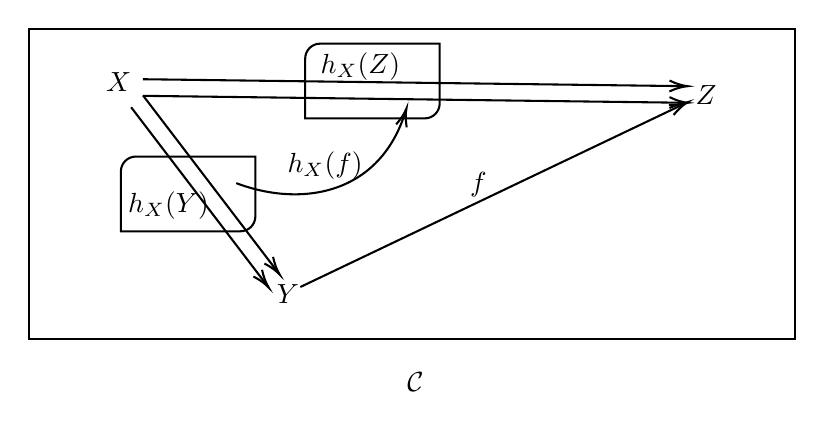
\begin{tikzpicture}[x=0.75pt,y=0.75pt,yscale=-1,xscale=1, scale = 0.8]
%uncomment if require: \path (0,300); %set diagram left start at 0, and has height of 300

%Shape: Rectangle [id:dp6898378251500559] 
\draw   (86,26) -- (547.5,26) -- (547.5,212.71) -- (86,212.71) -- cycle ;
%Rounded Diagonal Corner Rect [id:dp90110473299386] 
\draw   (141.5,112) .. controls (141.5,107.03) and (145.53,103) .. (150.5,103) -- (222.5,103) .. controls (222.5,103) and (222.5,103) .. (222.5,103) -- (222.5,139) .. controls (222.5,143.97) and (218.47,148) .. (213.5,148) -- (141.5,148) .. controls (141.5,148) and (141.5,148) .. (141.5,148) -- cycle ;
%Rounded Diagonal Corner Rect [id:dp20981670874217795] 
\draw   (252.5,44) .. controls (252.5,39.03) and (256.53,35) .. (261.5,35) -- (333.5,35) .. controls (333.5,35) and (333.5,35) .. (333.5,35) -- (333.5,71) .. controls (333.5,75.97) and (329.47,80) .. (324.5,80) -- (252.5,80) .. controls (252.5,80) and (252.5,80) .. (252.5,80) -- cycle ;
%Curve Lines [id:da18061312650610728] 
\draw    (211,119) .. controls (250.11,133.85) and (297.54,126.16) .. (313.04,75.55) ;
\draw [shift={(313.5,74)}, rotate = 106.09] [color={rgb, 255:red, 0; green, 0; blue, 0 }  ][line width=0.75]    (10.93,-3.29) .. controls (6.95,-1.4) and (3.31,-0.3) .. (0,0) .. controls (3.31,0.3) and (6.95,1.4) .. (10.93,3.29)   ;

% Text Node
\draw (312.19,231.45) node [anchor=north west][inner sep=0.75pt]    {$\mathcal{C}$};
% Text Node
\draw (130.81,50.69) node [anchor=north west][inner sep=0.75pt]    {$X$};
% Text Node
\draw (485.82,58.14) node [anchor=north west][inner sep=0.75pt]    {$Z$};
% Text Node
\draw (233.55,178.5) node [anchor=north west][inner sep=0.75pt]    {$Y$};
% Text Node
\draw (144,122.4) node [anchor=north west][inner sep=0.75pt]    {$h_{X}( Y)$};
% Text Node
\draw (350,110.4) node [anchor=north west][inner sep=0.75pt]    {$f$};
% Text Node
\draw (260,38.4) node [anchor=north west][inner sep=0.75pt]    {$h_{X}( Z)$};
% Text Node
\draw (240,98.4) node [anchor=north west][inner sep=0.75pt]    {$h_{X}( f)$};
% Connection
\draw    (154.81,66.16) -- (235.97,172.51) ;
\draw [shift={(237.18,174.1)}, rotate = 232.66] [color={rgb, 255:red, 0; green, 0; blue, 0 }  ][line width=0.75]    (10.93,-3.29) .. controls (6.95,-1.4) and (3.31,-0.3) .. (0,0) .. controls (3.31,0.3) and (6.95,1.4) .. (10.93,3.29)   ;
% Connection
\draw    (147.68,73.29) -- (229.33,180.31) ;
\draw [shift={(230.55,181.9)}, rotate = 232.66] [color={rgb, 255:red, 0; green, 0; blue, 0 }  ][line width=0.75]    (10.93,-3.29) .. controls (6.95,-1.4) and (3.31,-0.3) .. (0,0) .. controls (3.31,0.3) and (6.95,1.4) .. (10.93,3.29)   ;
% Connection
\draw    (154.81,56.42) -- (480.82,60.59) ;
\draw [shift={(482.82,60.62)}, rotate = 180.73] [color={rgb, 255:red, 0; green, 0; blue, 0 }  ][line width=0.75]    (10.93,-3.29) .. controls (6.95,-1.4) and (3.31,-0.3) .. (0,0) .. controls (3.31,0.3) and (6.95,1.4) .. (10.93,3.29)   ;
% Connection
\draw    (249.55,181.57) -- (481.01,71.13) ;
\draw [shift={(482.82,70.27)}, rotate = 154.49] [color={rgb, 255:red, 0; green, 0; blue, 0 }  ][line width=0.75]    (10.93,-3.29) .. controls (6.95,-1.4) and (3.31,-0.3) .. (0,0) .. controls (3.31,0.3) and (6.95,1.4) .. (10.93,3.29)   ;
% Connection
\draw    (154.81,66.42) -- (480.82,70.59) ;
\draw [shift={(482.82,70.62)}, rotate = 180.73] [color={rgb, 255:red, 0; green, 0; blue, 0 }  ][line width=0.75]    (10.93,-3.29) .. controls (6.95,-1.4) and (3.31,-0.3) .. (0,0) .. controls (3.31,0.3) and (6.95,1.4) .. (10.93,3.29)   ;

\end{tikzpicture}
    \end{figure}

$$\begin{array}{rrcl}
    h_X\left(\nu\circ\mu\right):&\mathcal{C}(X,Y) & \rightarrow &\mathcal{C}(X,W)\\
    & g &\rightarrow &\left(\nu\circ\mu\right)\circ g = \nu\circ \left(\mu\circ g\right)
\end{array}
$$
$$\mu\circ g = h_X(\mu)(g),$$

\begin{center}
\begin{tikzcd}
Y \arrow[r,  "\mu"] \arrow[dr,  swap,  "\nu\circ\mu"] &Z \arrow[d,  "\nu"] \\
& W
\end{tikzcd}
\end{center}
so,
$$\nu\circ\left(\mu\circ g\right) = h_X(\nu)\left(h_X(\mu)(g)\right),\ h_X(\nu\circ\mu) = h_X(\nu)\circ h_X(\mu).$$
\end{exampleenv}
\begin{exampleenv}
    Let $\mathcal{C}$ be a category. $\Id_\mathcal{C}$ that sends $X\in \Obj(C)$ to $X$ and $f:X\rightarrow Y$ to $f$. This is a functor.
\end{exampleenv}
\begin{exampleenv}
    Let $\mathcal{C}$, $\mathcal{D}$, $\mathcal{E}$ be categories, $F:\mathcal{C}\rightarrow\mathcal{D}$ and $G:\mathcal{D}\rightarrow\mathcal{E}$ be functors. We define a functor
    $$G\circ F:\mathcal{C}\rightarrow \mathcal{E}$$
    such that 
    $$\forall X\in \Obj(\mathcal{C}),\ \left(G\circ F\right)(X)=G(F(X)),$$
    $$\forall f:X\rightarrow Y,\ \left(G\circ F\right)(f) = G(F(f)).$$
\end{exampleenv}
\begin{definitionenv}
    Let $\mathcal{C}$ and $\mathcal{D}$ be categories, and $F:\mathcal{C}\rightarrow \mathcal{D}$ and $G:\mathcal{C}\rightarrow\mathcal{D}$ be functors. We call natural transformation (morphism of function) from $F$ to $G$ any family
    $$\varphi=\left(\varphi_X\right)_{X\in \Obj(\mathcal{C})}$$
    where $\varphi_X:F(X)\rightarrow G(X)$ is a morphism (in $\mathcal{D}$) such that for any morphism $f:X\rightarrow Y$ in $\mathcal{C}$, the following diagram is commutative:
    \begin{center}
    \begin{tikzcd}
F(X) \arrow[r,  "F(f)"] \arrow[d,  swap,  "\varphi_{X}"] &\displaystyle F(Y) \arrow[d,  "\varphi_Y"] \\
G(X) \arrow[r,"G(f)"]& G(Y)
\end{tikzcd}
\end{center}
$$G(f)\circ \varphi_X=\varphi_Y\circ F(f).$$
\begin{figure}[H]
    \centering


\tikzset{every picture/.style={line width=0.75pt}} %set default line width to 0.75pt        

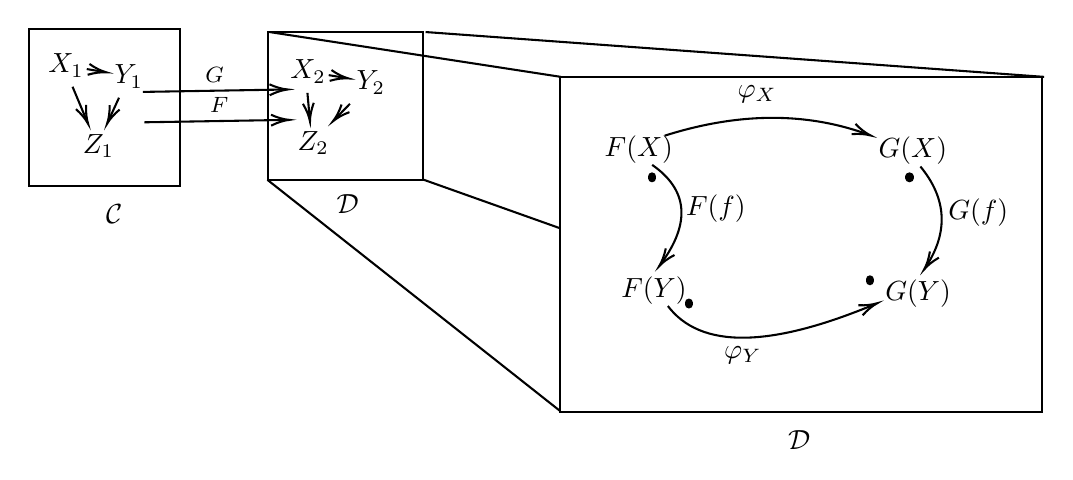
\begin{tikzpicture}[x=0.75pt,y=0.75pt,yscale=-1,xscale=1, scale = 0.8]
%uncomment if require: \path (0,300); %set diagram left start at 0, and has height of 300

%Shape: Rectangle [id:dp7089110550670655] 
\draw   (16,19) -- (107.31,19) -- (107.31,113.48) -- (16,113.48) -- cycle ;
%Shape: Rectangle [id:dp6149851284848306] 
\draw   (160.37,21.2) -- (253.5,21.2) -- (253.5,110.01) -- (160.37,110.01) -- cycle ;
%Straight Lines [id:da9596541637490664] 
\draw    (85.68,75.36) -- (170.89,73.93) ;
\draw [shift={(172.89,73.9)}, rotate = 179.04] [color={rgb, 255:red, 0; green, 0; blue, 0 }  ][line width=0.75]    (10.93,-3.29) .. controls (6.95,-1.4) and (3.31,-0.3) .. (0,0) .. controls (3.31,0.3) and (6.95,1.4) .. (10.93,3.29)   ;
%Straight Lines [id:da2100847392454801] 
\draw    (84.77,57.06) -- (169.98,55.63) ;
\draw [shift={(171.98,55.6)}, rotate = 179.04] [color={rgb, 255:red, 0; green, 0; blue, 0 }  ][line width=0.75]    (10.93,-3.29) .. controls (6.95,-1.4) and (3.31,-0.3) .. (0,0) .. controls (3.31,0.3) and (6.95,1.4) .. (10.93,3.29)   ;
%Shape: Rectangle [id:dp1302044156137787] 
\draw   (336,48) -- (626.5,48) -- (626.5,250) -- (336,250) -- cycle ;
%Straight Lines [id:da036506408298424] 
\draw    (159.78,110.02) -- (335.78,249.02) ;
%Straight Lines [id:da8328603435353752] 
\draw    (255,21) -- (627.5,48) ;
%Shape: Free Drawing [id:dp9920703584396833] 
\draw  [line width=3] [line join = round][line cap = round] (391.5,108) .. controls (391.5,108.33) and (391.5,108.67) .. (391.5,109) ;
%Shape: Free Drawing [id:dp7832409228988187] 
\draw  [line width=3] [line join = round][line cap = round] (546.5,108) .. controls (546.5,108.33) and (546.5,108.67) .. (546.5,109) ;
%Shape: Free Drawing [id:dp8584801540259973] 
\draw  [line width=3] [line join = round][line cap = round] (413.5,184) .. controls (413.5,184.33) and (413.5,184.67) .. (413.5,185) ;
%Shape: Free Drawing [id:dp8934882364262572] 
\draw  [line width=3] [line join = round][line cap = round] (522.5,170) .. controls (522.5,170.33) and (522.5,170.67) .. (522.5,171) ;
%Straight Lines [id:da8036087358907691] 
\draw    (254,110) -- (335.5,139) ;
%Straight Lines [id:da9261767614907577] 
\draw    (161,21) -- (336.5,48) ;

% Text Node
\draw (60.68,122.75) node [anchor=north west][inner sep=0.75pt]    {$\mathcal{C}$};
% Text Node
\draw (199.55,117.21) node [anchor=north west][inner sep=0.75pt]    {$\mathcal{D}$};
% Text Node
\draw (25.95,32.36) node [anchor=north west][inner sep=0.75pt]    {$X_{1}$};
% Text Node
\draw (65.84,38.95) node [anchor=north west][inner sep=0.75pt]    {$Y_{1}$};
% Text Node
\draw (46.72,80.67) node [anchor=north west][inner sep=0.75pt]    {$Z_{1}$};
% Text Node
\draw (171.68,36.02) node [anchor=north west][inner sep=0.75pt]    {$X_{2}$};
% Text Node
\draw (211.58,42.61) node [anchor=north west][inner sep=0.75pt]    {$Y_{2}$};
% Text Node
\draw (176.05,79.2) node [anchor=north west][inner sep=0.75pt]    {$Z_{2}$};
% Text Node
\draw (123.4,58.25) node [anchor=north west][inner sep=0.75pt]    {\footnotesize$F$};
% Text Node
\draw (120.58,40.68) node [anchor=north west][inner sep=0.75pt]    {\footnotesize$G$};
% Text Node
\draw (471.55,259.21) node [anchor=north west][inner sep=0.75pt]    {$\mathcal{D}$};
% Text Node
\draw (361,81.4) node [anchor=north west][inner sep=0.75pt]    {$F( X)$};
% Text Node
\draw (526,82.4) node [anchor=north west][inner sep=0.75pt]    {$G( X)$};
% Text Node
\draw (371,166.4) node [anchor=north west][inner sep=0.75pt]    {$F( Y)$};
% Text Node
\draw (530,168.4) node [anchor=north west][inner sep=0.75pt]    {$G( Y)$};
% Text Node
\draw (441,51.4) node [anchor=north west][inner sep=0.75pt]    {$\varphi _{X}$};
% Text Node
\draw (433,208.4) node [anchor=north west][inner sep=0.75pt]    {$\varphi _{Y}$};
% Text Node
\draw (410,117.4) node [anchor=north west][inner sep=0.75pt]    {$F( f)$};
% Text Node
\draw (568,119.4) node [anchor=north west][inner sep=0.75pt]    {$G( f)$};
% Connection
\draw    (42.4,53.96) -- (50.99,74.42) ;
\draw [shift={(51.76,76.27)}, rotate = 247.24] [color={rgb, 255:red, 0; green, 0; blue, 0 }  ][line width=0.75]    (10.93,-3.29) .. controls (6.95,-1.4) and (3.31,-0.3) .. (0,0) .. controls (3.31,0.3) and (6.95,1.4) .. (10.93,3.29)   ;
% Connection
\draw    (50.95,43.3) -- (60.87,44.96) ;
\draw [shift={(62.84,45.29)}, rotate = 189.49] [color={rgb, 255:red, 0; green, 0; blue, 0 }  ][line width=0.75]    (10.93,-3.29) .. controls (6.95,-1.4) and (3.31,-0.3) .. (0,0) .. controls (3.31,0.3) and (6.95,1.4) .. (10.93,3.29)   ;
% Connection
\draw    (70.38,60.55) -- (64.01,74.45) ;
\draw [shift={(63.18,76.27)}, rotate = 294.63] [color={rgb, 255:red, 0; green, 0; blue, 0 }  ][line width=0.75]    (10.93,-3.29) .. controls (6.95,-1.4) and (3.31,-0.3) .. (0,0) .. controls (3.31,0.3) and (6.95,1.4) .. (10.93,3.29)   ;
% Connection
\draw    (183.85,57.62) -- (185.21,72.81) ;
\draw [shift={(185.39,74.8)}, rotate = 264.88] [color={rgb, 255:red, 0; green, 0; blue, 0 }  ][line width=0.75]    (10.93,-3.29) .. controls (6.95,-1.4) and (3.31,-0.3) .. (0,0) .. controls (3.31,0.3) and (6.95,1.4) .. (10.93,3.29)   ;
% Connection
\draw    (196.68,46.96) -- (206.6,48.62) ;
\draw [shift={(208.58,48.95)}, rotate = 189.49] [color={rgb, 255:red, 0; green, 0; blue, 0 }  ][line width=0.75]    (10.93,-3.29) .. controls (6.95,-1.4) and (3.31,-0.3) .. (0,0) .. controls (3.31,0.3) and (6.95,1.4) .. (10.93,3.29)   ;
% Connection
\draw    (209.46,64.21) -- (200.56,73.37) ;
\draw [shift={(199.17,74.8)}, rotate = 314.15] [color={rgb, 255:red, 0; green, 0; blue, 0 }  ][line width=0.75]    (10.93,-3.29) .. controls (6.95,-1.4) and (3.31,-0.3) .. (0,0) .. controls (3.31,0.3) and (6.95,1.4) .. (10.93,3.29)   ;
% Connection
\draw    (399,83.43) .. controls (443.33,69.35) and (484.09,69.09) .. (521.3,82.65) ;
\draw [shift={(523,83.28)}, rotate = 200.64] [color={rgb, 255:red, 0; green, 0; blue, 0 }  ][line width=0.75]    (10.93,-3.29) .. controls (6.95,-1.4) and (3.31,-0.3) .. (0,0) .. controls (3.31,0.3) and (6.95,1.4) .. (10.93,3.29)   ;
% Connection
\draw    (400.92,186) .. controls (420.54,211.87) and (462.25,211.44) .. (526.04,184.73) ;
\draw [shift={(527,184.32)}, rotate = 157.14] [color={rgb, 255:red, 0; green, 0; blue, 0 }  ][line width=0.75]    (10.93,-3.29) .. controls (6.95,-1.4) and (3.31,-0.3) .. (0,0) .. controls (3.31,0.3) and (6.95,1.4) .. (10.93,3.29)   ;
% Connection
\draw    (391.47,101) .. controls (413.05,116.02) and (414.84,135.86) .. (396.82,160.49) ;
\draw [shift={(395.69,162)}, rotate = 307.18] [color={rgb, 255:red, 0; green, 0; blue, 0 }  ][line width=0.75]    (10.93,-3.29) .. controls (6.95,-1.4) and (3.31,-0.3) .. (0,0) .. controls (3.31,0.3) and (6.95,1.4) .. (10.93,3.29)   ;
% Connection
\draw    (553.03,102) .. controls (568.91,121.33) and (570.01,141.47) .. (556.33,162.39) ;
\draw [shift={(555.25,164)}, rotate = 304.57] [color={rgb, 255:red, 0; green, 0; blue, 0 }  ][line width=0.75]    (10.93,-3.29) .. controls (6.95,-1.4) and (3.31,-0.3) .. (0,0) .. controls (3.31,0.3) and (6.95,1.4) .. (10.93,3.29)   ;

\end{tikzpicture}
\end{figure}
\end{definitionenv}
\begin{exampleenv}
    Let $\Id_F$ be the family $\left(\Id_{F(X)}\right)_{X\in \Obj(\mathcal{C})}$. This is a morphism of functors from $F$ to $F$, called the identity morphism.
    \begin{center}
    \begin{tikzcd}
F(X) \arrow[r,  "F(f)"] \arrow[d,  swap,  "\Id_{F(X)}"] &\displaystyle F(Y) \arrow[d,  "\Id_{F(Y)}"] \\
F(X) \arrow[r,"F(f)"]& F(Y)
\end{tikzcd}
\end{center}
$$F(f)\circ \Id_{F(X)} = F(f) =\Id_{F(Y)}\circ F(f).$$
\end{exampleenv}
\begin{exampleenv}
    Let $F$, $G$ and $H$ be functors from $\mathcal{C}$ to $\mathcal{D}$, $\varphi: F\rightarrow G$, $\psi:G\rightarrow H$ be natural transformations. We define
    $$\psi\circ \varphi: F\rightarrow H$$
    as the family 
    $$ \left(\psi_X\circ\varphi_X\right)_{X\in \Obj(\mathcal{C})},\ F(X)\overset{\varphi_X}{\longrightarrow}G(X)\overset{\psi_X}{\longrightarrow}H(X).$$
    It is called the composite of $\psi$ and $\varphi$.
\end{exampleenv}
\begin{remark}
    Let $\mathcal{C}$ and $\mathcal{D}$ be categories. Let $\underline{\mathrm{Fun}}(\mathcal{C},\mathcal{D})$ be the data that is composite of
    \begin{itemize}
        \item The set of all functors from $\mathcal{C}$ to $\mathcal{D}$
        \item Natural transformations.
    \end{itemize}
    Then $\underline{\mathrm{Fun}}(\mathcal{C},\mathcal{D})$ forms a category (in some suitable universe). It is called the category of functors from $\mathcal{C}$ to $\mathcal{D}$. If $F$ and $G$ are two functors from $\mathcal{C}$ to $\mathcal{D}$ such that there exists an isomorphism from $F$ to $G$ in $\underline{\mathrm{Fun}}(\mathcal{C},\mathcal{D})$. We say that $F$ and $G$ are isomorphic.
\end{remark}
\begin{propositionenv}
    Let $\mathcal{U}$ be a universe, $\mathcal{C}$ be a $\mathcal{U}$-small category, and $\mathcal{D}$ be a $\mathcal{U}$-category. For any functors $F$ and $G$ from $\mathcal{C}$ to $\mathcal{D}$, the set $\mathrm{Nat}(F,G)$ of natural transformation from $F$ to $G$ belongs to $\mathcal{U}$.
\end{propositionenv}
\begin{proofenv}
    $\mathrm{Nat}(F,G)$ is a subset of $\dis \prod_{X\in \Obj(\mathcal{C})}\mathcal{D}(F(X),G(X))\in \mathcal{U}$.
\end{proofenv}
\begin{notationenv}
    If $\mathcal{C}$ is a category, then $\underline{\mathrm{Fun}}(\mathcal{C},\underline{\mathrm{Set}})$ is denoted by $\hat{\mathcal{C}}$.
\end{notationenv}
\newpage
\section{Yoneda Lemma}
\begin{theoremenv}
    Let $\mathcal{C}$ be a category, $F:\mathcal{C}\rightarrow \underline{\mathrm{Set}}$ be a functor and $X\in \Obj(\mathcal{C})$. Then
    $$\begin{array}{rrcl}
        \beta:&\mathrm{Nat}(h_X,F)&\rightarrow& F(X)\\
        & \psi&\mapsto&\psi_X(\Id_X)\footnote{$\psi_X:h_X(X)=\mathcal{C}(X,X)\rightarrow F(X)$.}
    \end{array}$$
    is a bijection.
    \begin{figure}[H]
    \centering


\tikzset{every picture/.style={line width=0.75pt}} %set default line width to 0.75pt        

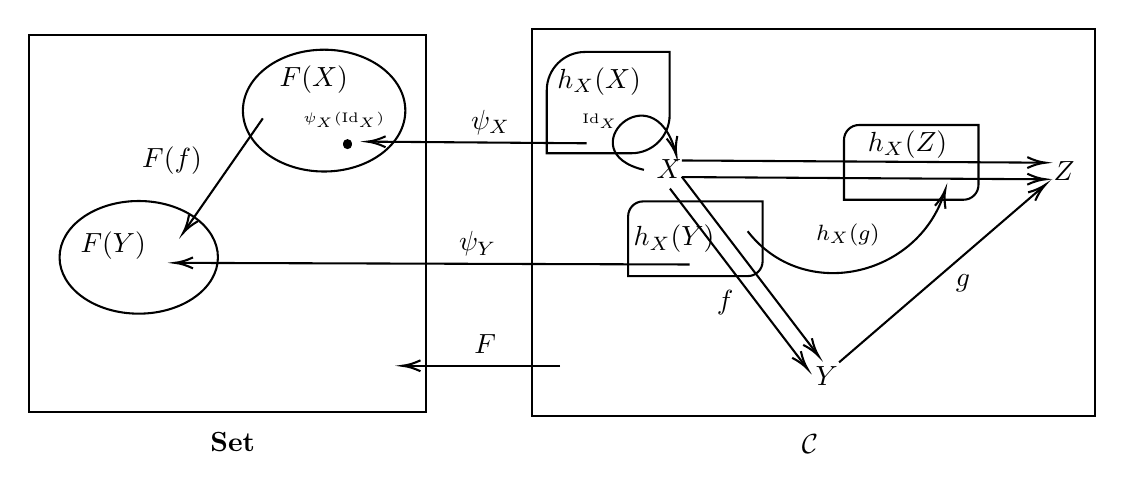
\begin{tikzpicture}[x=0.75pt,y=0.75pt,yscale=-1,xscale=1, scale =0.8]
%uncomment if require: \path (0,300); %set diagram left start at 0, and has height of 300

%Shape: Rectangle [id:dp29104558201405406] 
\draw   (314.5,30) -- (653.5,30) -- (653.5,263) -- (314.5,263) -- cycle ;
%Rounded Diagonal Corner Rect [id:dp44417459474777166] 
\draw   (372.5,143) .. controls (372.5,138.03) and (376.53,134) .. (381.5,134) -- (453.5,134) .. controls (453.5,134) and (453.5,134) .. (453.5,134) -- (453.5,170) .. controls (453.5,174.97) and (449.47,179) .. (444.5,179) -- (372.5,179) .. controls (372.5,179) and (372.5,179) .. (372.5,179) -- cycle ;
%Rounded Diagonal Corner Rect [id:dp5510703091888516] 
\draw   (502.5,97) .. controls (502.5,92.03) and (506.53,88) .. (511.5,88) -- (583.5,88) .. controls (583.5,88) and (583.5,88) .. (583.5,88) -- (583.5,124) .. controls (583.5,128.97) and (579.47,133) .. (574.5,133) -- (502.5,133) .. controls (502.5,133) and (502.5,133) .. (502.5,133) -- cycle ;
%Curve Lines [id:da6732018462293708] 
\draw    (444.5,152) .. controls (478.16,195.56) and (547.1,179.33) .. (563.03,128.55) ;
\draw [shift={(563.5,127)}, rotate = 106.09] [color={rgb, 255:red, 0; green, 0; blue, 0 }  ][line width=0.75]    (10.93,-3.29) .. controls (6.95,-1.4) and (3.31,-0.3) .. (0,0) .. controls (3.31,0.3) and (6.95,1.4) .. (10.93,3.29)   ;
%Shape: Rectangle [id:dp49619736846033] 
\draw   (11.5,34) -- (250.5,34) -- (250.5,261) -- (11.5,261) -- cycle ;
%Shape: Ellipse [id:dp5211352656838969] 
\draw   (140.5,79.32) .. controls (140.5,59.06) and (162.4,42.64) .. (189.4,42.64) .. controls (216.41,42.64) and (238.31,59.06) .. (238.31,79.32) .. controls (238.31,99.58) and (216.41,116) .. (189.4,116) .. controls (162.4,116) and (140.5,99.58) .. (140.5,79.32) -- cycle ;
%Straight Lines [id:da796610559906879] 
\draw    (331.5,233) -- (238.5,233) ;
\draw [shift={(236.5,233)}, rotate = 360] [color={rgb, 255:red, 0; green, 0; blue, 0 }  ][line width=0.75]    (10.93,-3.29) .. controls (6.95,-1.4) and (3.31,-0.3) .. (0,0) .. controls (3.31,0.3) and (6.95,1.4) .. (10.93,3.29)   ;
%Shape: Ellipse [id:dp4066346829093145] 
\draw   (30.08,167.69) .. controls (30.08,148.95) and (51.43,133.76) .. (77.76,133.76) .. controls (104.1,133.76) and (125.45,148.95) .. (125.45,167.69) .. controls (125.45,186.42) and (104.1,201.61) .. (77.76,201.61) .. controls (51.43,201.61) and (30.08,186.42) .. (30.08,167.69) -- cycle ;
%Rounded Diagonal Corner Rect [id:dp9719492308142043] 
\draw   (323.5,67.04) .. controls (323.5,54.32) and (333.82,44) .. (346.54,44) -- (397.5,44) .. controls (397.5,44) and (397.5,44) .. (397.5,44) -- (397.5,81.96) .. controls (397.5,94.68) and (387.18,105) .. (374.46,105) -- (323.5,105) .. controls (323.5,105) and (323.5,105) .. (323.5,105) -- cycle ;
%Curve Lines [id:da2752984146564955] 
\draw    (382,115) .. controls (335.97,104.11) and (387.45,54.02) .. (401.1,104.44) ;
\draw [shift={(401.5,106)}, rotate = 256.22] [color={rgb, 255:red, 0; green, 0; blue, 0 }  ][line width=0.75]    (10.93,-3.29) .. controls (6.95,-1.4) and (3.31,-0.3) .. (0,0) .. controls (3.31,0.3) and (6.95,1.4) .. (10.93,3.29)   ;
%Straight Lines [id:da19731840968168723] 
\draw    (347.5,99) -- (217.5,98.02) ;
\draw [shift={(215.5,98)}, rotate = 0.43] [color={rgb, 255:red, 0; green, 0; blue, 0 }  ][line width=0.75]    (10.93,-3.29) .. controls (6.95,-1.4) and (3.31,-0.3) .. (0,0) .. controls (3.31,0.3) and (6.95,1.4) .. (10.93,3.29)   ;
%Shape: Free Drawing [id:dp2493761350192819] 
\draw  [line width=3] [line join = round][line cap = round] (203.5,99) .. controls (203.5,99.33) and (203.5,99.67) .. (203.5,100) ;
%Straight Lines [id:da5093037449359683] 
\draw    (409.5,172) -- (101.5,171.01) ;
\draw [shift={(99.5,171)}, rotate = 0.18] [color={rgb, 255:red, 0; green, 0; blue, 0 }  ][line width=0.75]    (10.93,-3.29) .. controls (6.95,-1.4) and (3.31,-0.3) .. (0,0) .. controls (3.31,0.3) and (6.95,1.4) .. (10.93,3.29)   ;
%Straight Lines [id:da8188395842578471] 
\draw    (152.5,84) -- (105.64,151.36) ;
\draw [shift={(104.5,153)}, rotate = 304.82] [color={rgb, 255:red, 0; green, 0; blue, 0 }  ][line width=0.75]    (10.93,-3.29) .. controls (6.95,-1.4) and (3.31,-0.3) .. (0,0) .. controls (3.31,0.3) and (6.95,1.4) .. (10.93,3.29)   ;

% Text Node
\draw (475.19,272.45) node [anchor=north west][inner sep=0.75pt]    {$\mathcal{C}$};
% Text Node
\draw (387.81,106.69) node [anchor=north west][inner sep=0.75pt]    {$X$};
% Text Node
\draw (626.82,108.14) node [anchor=north west][inner sep=0.75pt]    {$Z$};
% Text Node
\draw (483.55,231.5) node [anchor=north west][inner sep=0.75pt]    {$Y$};
% Text Node
\draw (374,146.4) node [anchor=north west][inner sep=0.75pt]    {$h_{X}( Y)$};
% Text Node
\draw (568,176.4) node [anchor=north west][inner sep=0.75pt]    {$g$};
% Text Node
\draw (515,89.4) node [anchor=north west][inner sep=0.75pt]    {$h_{X}( Z)$};
% Text Node
\draw (484,145.4) node [anchor=north west][inner sep=0.75pt]    {\footnotesize$h_{X}( g)$};
% Text Node
\draw (119,271.4) node [anchor=north west][inner sep=0.75pt]    {$\mathbf{Set}$};
% Text Node
\draw (278,212.4) node [anchor=north west][inner sep=0.75pt]    {$F$};
% Text Node
\draw (160.74,50.52) node [anchor=north west][inner sep=0.75pt]    {$F( X)$};
% Text Node
\draw (40.85,150.65) node [anchor=north west][inner sep=0.75pt]    {$F( Y)$};
% Text Node
\draw (328,51.4) node [anchor=north west][inner sep=0.75pt]    {$h_{X}( X)$};
% Text Node
\draw (276,77.4) node [anchor=north west][inner sep=0.75pt]    {$\psi _{X}$};
% Text Node
\draw (343,79.4) node [anchor=north west][inner sep=0.75pt]    {\tiny$\mathrm{Id}_{X}$};
% Text Node
\draw (175,78.4) node [anchor=north west][inner sep=0.75pt]    {\tiny$\psi _{X}(\mathrm{Id}_{X})$};
% Text Node
\draw (268.77,150.4) node [anchor=north west][inner sep=0.75pt]    {$\psi _{Y}$};
% Text Node
\draw (424,185.4) node [anchor=north west][inner sep=0.75pt]    {$f$};
% Text Node
\draw (78,99.4) node [anchor=north west][inner sep=0.75pt]    {$F( f)$};
% Connection
\draw    (404.81,119.16) -- (485.97,225.51) ;
\draw [shift={(487.18,227.1)}, rotate = 232.66] [color={rgb, 255:red, 0; green, 0; blue, 0 }  ][line width=0.75]    (10.93,-3.29) .. controls (6.95,-1.4) and (3.31,-0.3) .. (0,0) .. controls (3.31,0.3) and (6.95,1.4) .. (10.93,3.29)   ;
% Connection
\draw    (397.68,126.29) -- (479.33,233.31) ;
\draw [shift={(480.55,234.9)}, rotate = 232.66] [color={rgb, 255:red, 0; green, 0; blue, 0 }  ][line width=0.75]    (10.93,-3.29) .. controls (6.95,-1.4) and (3.31,-0.3) .. (0,0) .. controls (3.31,0.3) and (6.95,1.4) .. (10.93,3.29)   ;
% Connection
\draw    (404.81,109.35) -- (621.82,110.67) ;
\draw [shift={(623.82,110.68)}, rotate = 180.35] [color={rgb, 255:red, 0; green, 0; blue, 0 }  ][line width=0.75]    (10.93,-3.29) .. controls (6.95,-1.4) and (3.31,-0.3) .. (0,0) .. controls (3.31,0.3) and (6.95,1.4) .. (10.93,3.29)   ;
% Connection
\draw    (499.55,230.92) -- (622.3,125.22) ;
\draw [shift={(623.82,123.92)}, rotate = 139.27] [color={rgb, 255:red, 0; green, 0; blue, 0 }  ][line width=0.75]    (10.93,-3.29) .. controls (6.95,-1.4) and (3.31,-0.3) .. (0,0) .. controls (3.31,0.3) and (6.95,1.4) .. (10.93,3.29)   ;
% Connection
\draw    (404.81,119.35) -- (621.82,120.67) ;
\draw [shift={(623.82,120.68)}, rotate = 180.35] [color={rgb, 255:red, 0; green, 0; blue, 0 }  ][line width=0.75]    (10.93,-3.29) .. controls (6.95,-1.4) and (3.31,-0.3) .. (0,0) .. controls (3.31,0.3) and (6.95,1.4) .. (10.93,3.29)   ;

\end{tikzpicture}
    \end{figure}
\end{theoremenv}
\begin{proofenv}
    We construct a mapping
    $$\begin{array}{rrcl}
        \alpha:&F(X)&\rightarrow&\mathrm{Nat}(h_X,F)\\
        &x&\mapsto&\alpha(x)=(\alpha(x)_Y)_{Y\in \Obj(\mathcal{C})}
    \end{array}
    $$
    \begin{figure}[H]
    \centering
\tikzset{every picture/.style={line width=0.75pt}} %set default line width to 0.75pt        

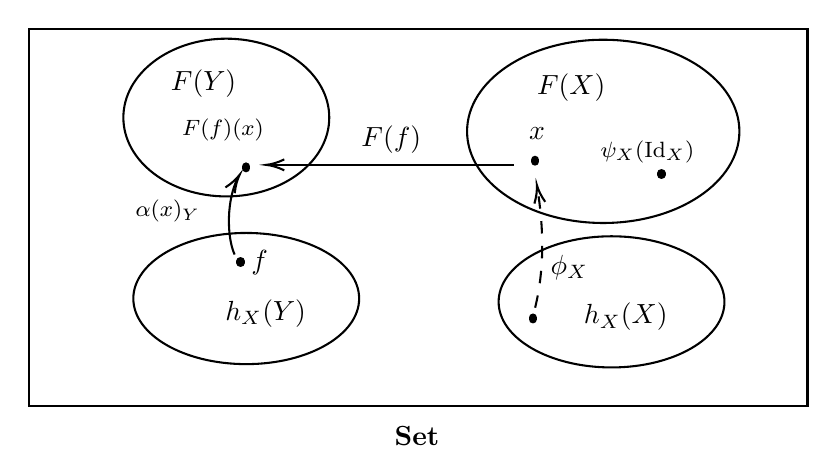
\begin{tikzpicture}[x=0.75pt,y=0.75pt,yscale=-1,xscale=1, scale = 0.8]
%uncomment if require: \path (0,300); %set diagram left start at 0, and has height of 300

%Shape: Rectangle [id:dp19892027739488838] 
\draw   (94.5,26) -- (563.5,26) -- (563.5,253) -- (94.5,253) -- cycle ;
%Shape: Ellipse [id:dp35634985592370083] 
\draw   (358.5,87.82) .. controls (358.5,57.34) and (395.21,32.64) .. (440.5,32.64) .. controls (485.79,32.64) and (522.5,57.34) .. (522.5,87.82) .. controls (522.5,118.29) and (485.79,143) .. (440.5,143) .. controls (395.21,143) and (358.5,118.29) .. (358.5,87.82) -- cycle ;
%Shape: Ellipse [id:dp7145581050737746] 
\draw   (151.5,79.5) .. controls (151.5,53.27) and (179.26,32) .. (213.5,32) .. controls (247.74,32) and (275.5,53.27) .. (275.5,79.5) .. controls (275.5,105.73) and (247.74,127) .. (213.5,127) .. controls (179.26,127) and (151.5,105.73) .. (151.5,79.5) -- cycle ;
%Shape: Free Drawing [id:dp5680895793130827] 
\draw  [line width=3] [line join = round][line cap = round] (475.5,113) .. controls (475.5,113.33) and (475.5,113.67) .. (475.5,114) ;
%Straight Lines [id:da4515185175819256] 
\draw    (386.5,108) -- (239.5,108) ;
\draw [shift={(237.5,108)}, rotate = 360] [color={rgb, 255:red, 0; green, 0; blue, 0 }  ][line width=0.75]    (10.93,-3.29) .. controls (6.95,-1.4) and (3.31,-0.3) .. (0,0) .. controls (3.31,0.3) and (6.95,1.4) .. (10.93,3.29)   ;
%Shape: Free Drawing [id:dp8664607428198391] 
\draw  [line width=3] [line join = round][line cap = round] (399.5,105) .. controls (399.5,105.33) and (399.5,105.67) .. (399.5,106) ;
%Shape: Free Drawing [id:dp8705631504135898] 
\draw  [line width=3] [line join = round][line cap = round] (225.5,109) .. controls (225.5,109.33) and (225.5,109.67) .. (225.5,110) ;
%Curve Lines [id:da06385969038265649] 
\draw  [dash pattern={on 4.5pt off 4.5pt}]  (399.5,194) .. controls (405.35,169.62) and (404.55,145.25) .. (400.79,121.8) ;
\draw [shift={(400.5,120)}, rotate = 80.54] [color={rgb, 255:red, 0; green, 0; blue, 0 }  ][line width=0.75]    (10.93,-3.29) .. controls (6.95,-1.4) and (3.31,-0.3) .. (0,0) .. controls (3.31,0.3) and (6.95,1.4) .. (10.93,3.29)   ;
%Shape: Ellipse [id:dp6467487281921943] 
\draw   (377.5,190.5) .. controls (377.5,168.68) and (407.94,151) .. (445.5,151) .. controls (483.06,151) and (513.5,168.68) .. (513.5,190.5) .. controls (513.5,212.32) and (483.06,230) .. (445.5,230) .. controls (407.94,230) and (377.5,212.32) .. (377.5,190.5) -- cycle ;
%Shape: Ellipse [id:dp4928430640278725] 
\draw   (157.5,188.5) .. controls (157.5,166.68) and (187.94,149) .. (225.5,149) .. controls (263.06,149) and (293.5,166.68) .. (293.5,188.5) .. controls (293.5,210.32) and (263.06,228) .. (225.5,228) .. controls (187.94,228) and (157.5,210.32) .. (157.5,188.5) -- cycle ;
%Shape: Free Drawing [id:dp819965093523772] 
\draw  [line width=3] [line join = round][line cap = round] (222.09,166) .. controls (222.09,166.33) and (222.09,166.67) .. (222.09,167) ;
%Curve Lines [id:da9112028098270881] 
\draw    (218.5,162) .. controls (213.7,151.44) and (213.51,128.9) .. (220.58,115.61) ;
\draw [shift={(221.5,114)}, rotate = 121.61] [color={rgb, 255:red, 0; green, 0; blue, 0 }  ][line width=0.75]    (10.93,-3.29) .. controls (6.95,-1.4) and (3.31,-0.3) .. (0,0) .. controls (3.31,0.3) and (6.95,1.4) .. (10.93,3.29)   ;
%Shape: Free Drawing [id:dp6961614065798236] 
\draw  [line width=3] [line join = round][line cap = round] (398.09,200) .. controls (398.09,200.33) and (398.09,200.67) .. (398.09,201) ;

% Text Node
\draw (313,263.4) node [anchor=north west][inner sep=0.75pt]    {$\mathbf{Set}$};
% Text Node
\draw (398.74,51.52) node [anchor=north west][inner sep=0.75pt]    {$F( X)$};
% Text Node
\draw (178.24,48.76) node [anchor=north west][inner sep=0.75pt]    {$F( Y)$};
% Text Node
\draw (437,91.4) node [anchor=north west][inner sep=0.75pt]    {\footnotesize$\psi _{X}(\mathrm{Id}_{X})$};
% Text Node
\draw (293,82.4) node [anchor=north west][inner sep=0.75pt]    {$F( f)$};
% Text Node
\draw (394,83.4) node [anchor=north west][inner sep=0.75pt]    {$x$};
% Text Node
\draw (185,78.4) node [anchor=north west][inner sep=0.75pt]    {\footnotesize$F( f)( x)$};
% Text Node
\draw (407,160.4) node [anchor=north west][inner sep=0.75pt]    {$\phi _{X}$};
% Text Node
\draw (427,189.4) node [anchor=north west][inner sep=0.75pt]    {$h_{X}( X)$};
% Text Node
\draw (211,187.4) node [anchor=north west][inner sep=0.75pt]    {$h_{X}( Y)$};
% Text Node
\draw (226.75,157.4) node [anchor=north west][inner sep=0.75pt]    {$f$};
% Text Node
\draw (157,127.4) node [anchor=north west][inner sep=0.75pt]    {\footnotesize$\alpha ( x)_{Y}$};


\end{tikzpicture}
\end{figure}
    where $\alpha(x)_{Y}:h_X(Y)=\mathcal{C}(X,Y)\rightarrow F(Y)$, $f\mapsto F(f)(x)$. We need to check that $\alpha(x)$ is a natural transformation.
    Namely, for any $ \mu:A\rightarrow B$ in $\mathcal{C}$, we have a commutative diagram
    \begin{center}
    \begin{tikzcd}
\mathcal{C}(X,A) \arrow[d, swap, "\alpha(x)_A"]  \arrow[r, "h_X(\mu)"]& \mathcal{C}(X,B) \arrow[d,  "\alpha(x)_B"] \\
F(A) \arrow[r,"F(\mu)"]& F(B)  
\end{tikzcd}
\end{center}
In fact, 
$\forall f\in \mathcal{C}(X,A)$, $$\alpha(x)_B(h_X(\mu)(f))=\alpha(x)_B(\mu\circ f)=F(\mu\circ f)(x),$$
$$F(\mu)\left(\alpha(x)_A(f)\right) = F(\mu)\left(F(f)(x)\right)=F(\mu\circ f)(x).$$
We then check that $\alpha$ and $\beta$ are inverse of each other.
\begin{itemize}
    \item Let $\psi:h_X\rightarrow F$ be a natural transformation and $x=\psi_X(\Id_X)$. For any $f:X\rightarrow Y$ in $\mathcal{C}$,
    $$\alpha(x)_{Y}(f) = F(f)(x) = F(f)\left(\psi_X(\Id_X)\right)=\psi_Y\left(h_X(f)(\Id_X)\right)=\psi_Y(f).$$
    So, $\alpha(x)=\psi$.
    \item For any $x\in F(x)$,
    $$ \beta\left(\alpha(x)\right)=\alpha(x)_X\left(\Id_X\right)= F(\Id_X)(x) = \Id_{F(X)}(x)=x.$$
\end{itemize}
    \begin{center}
    \begin{tikzcd}
h_X(X) \arrow[r,  "F(f)"] \arrow[d,  swap,  "\psi_X"] &\displaystyle F(Y) \arrow[d,  "\psi_Y"] \\
F(X) \arrow[r,"F(f)"]& F(Y)
\end{tikzcd}
\end{center}
\end{proofenv}
\begin{notationenv}
    Let $\mathcal{C}$ be a category, and $f:Y\rightarrow X$ be a morphism in $\mathcal{C}$. By the theorem, we have a bijection
    $$\begin{array}{rcl}
        \mathrm{Nat}(h_X,h_Y)&\rightarrow &h_Y(X)=\mathcal{C}(Y,X)\\
        \psi&\mapsto&\psi_X(\Id_X).
    \end{array}$$
    We denote by $\upsilon(f):h_X\rightarrow h_Y$ the natural transformation that corresponds to $f$ by this bijection. ($\upsilon(f)= \left(\upsilon(f)_Z\right)_{Z\in \Obj(\mathcal{C})}$)
    $$ \begin{array}{rrcl}
        \upsilon(f)_{Z} :& \mathcal{C}(X,Z)&\rightarrow&\mathcal{C}(Y,Z)\\
        &\mu&\mapsto& h_Y(\mu)(f)=\mu\circ f.
    \end{array}
    $$
\end{notationenv}
\begin{propositionenv}
    $\upsilon: \mathcal{C}^{\op}\rightarrow\hat{\mathcal{C}}$ is a functor.
\end{propositionenv}
\begin{proofenv}
    Let $X\in \Obj(\mathcal{C})$. For any $Z\in \Obj(\mathcal{C})$
    $$\begin{array}{rrcl}
        \Id_{\mathcal{C}(X,Z)}=\upsilon(\Id_{X})_Z:&\mathcal{C}(X,Z)&\rightarrow&\mathcal{C}(X,Z)\\
        &\mu&\mapsto&\mu\circ\Id_X=\mu.
    \end{array}
    $$
    Let $Z\overset{g}{\longrightarrow}Y\overset{f}{\longrightarrow}X$ be morphisms in $\mathcal{C}$.
    $$g\circ_{\mathcal{C}^\op} f=f\circ_{\mathcal{C}} g.$$
    $$\begin{array}{rrcl}
        \upsilon\left(g\circ_{\mathcal{C}^\op} f\right)_{W}= \upsilon\left(f\circ_{\mathcal{C}}g\right)_{W} :& \mathcal{C}(X,W)&\rightarrow &\mathcal{C}(Z,W)\\
        &\mu &\mapsto & \mu\circ \left(f\circ g\right)= \left(\mu\circ f\right)\circ g.
    \end{array}
    $$
    $$\upsilon(g)\left(\upsilon(f)(\mu)\right) = \upsilon(g)\left(\mu\circ f\right) = \left(\mu\circ f\right)\circ g.$$
\end{proofenv}
\begin{propositionenv}
    Let $\mathcal{C}$ be a category and $f:Y\rightarrow X$ be a morphism. Then $f$ is an isomorphism if and only if $\upsilon(f)$ is an isomorphism in $\hat{\mathcal{C}}$.

    Moreover, $$\upsilon(f)^{-1} = \upsilon(f^{-1}).$$
\end{propositionenv}
\begin{proofenv}\quad \newline
    ``$\Rightarrow$'' If $f$ is an isomorphism,
    $$ \upsilon(f)\circ \upsilon(f^{-1}) = \upsilon(f^{-1}\circ f) = \upsilon(\Id_Y) = \Id_{h_Y},$$
    $$ \upsilon(f^{-1})\circ \upsilon(f) = \upsilon(f\circ f^{-1}) = \upsilon(\Id_X) =\Id_{h_X}.$$
    ``$\Leftarrow$'' If $\upsilon(f)$ if invertible and $\varphi = \upsilon(f)^{-1}$. Let $g:y\rightarrow X$ such that $\varphi=\upsilon(g)$.
    $$\upsilon(f\circ g) =\upsilon(g)\circ \upsilon(f) =\Id_{h_X},$$
    $$\upsilon(g\circ f) = \upsilon(f)\circ \upsilon(g) = \Id_{h_Y}.$$
\end{proofenv}
\newpage
\section{Representable Functors}
\begin{definitionenv}
    Let $\mathcal{C}$ be a category, $F:\mathcal{C}\rightarrow\underline{\mathrm{Set}}$ be a functor.
    
    \quad If there exists an object $X$ in $\mathcal{C}$ such that $F$ and $h_X$ are isomorphic, then we say that the functor $F$ is \textbf{representable} and $X$ is an object that represents the functor $F$.
    
    \quad An isomorphism from $h_X$ to $F$ is called a \textbf{representation} of the functor $F$ by the object $X$.

    \quad Let $F:\mathcal{C}\rightarrow \set$ be a representable functor and $X\in \mathcal{C}$ be an object that represents $F$. Let $\psi: h_X\rightarrow F$ be an isomorphism (of functors). Then the element $\psi_X\left(\Id_X\right)\in F(X)$ is called the \textbf{universal object} of the representation $\psi$.
\end{definitionenv}
\begin{propositionenv}\label{1.5.2}
    Let $\mathcal{C}$ be a category, $F:\mathcal{C}\rightarrow\set$ be a functor. Assume that $F$ is representable by $X\in \mathcal{C}$ and $\varphi:h_X \rightarrow F$ be the representing isomorphism. Denote $x$ the universal object of $\varphi$
    $$ x\coloneq \varphi_X\left(\Id_X\right).$$
    Then for any $Y\in \Obj(\mathcal{C})$ and any $y\in F(Y)$, there exists a unique morphism $f:X\rightarrow Y$ such that
    $$
    F(f)(x) = y.
    $$
    Actually, the morphism $f$ is given by $\varphi^{-1}_{Y}(y)$.
\end{propositionenv}
\begin{proofenv}
    Uniqueness: 
\begin{center}
\begin{tikzcd}
h_X(X) \arrow[r,  "\varphi_X"] \arrow[d,  swap,  "h_X (f)"] &F(X) \arrow[d,  "F(f)"] \\
h_X(Y) \arrow[r,"\varphi_Y"]& F(Y)
\end{tikzcd}
\end{center}
can be also written as
\begin{center}
\begin{tikzcd}
\mathcal{C}(X,X) \arrow[r,  "\varphi_X"] \arrow[d,  swap,  "f\circ(\ )"] &F(X) \arrow[d,  "F(f)"] \\
\mathcal{C}(X,Y) \arrow[r,"\varphi_Y"]& F(Y)
\end{tikzcd}
\end{center}
$$
y = F(f)(x) = F(f) \left(\varphi_X(\Id_X)\right) =\varphi_Y\left(f\circ\Id_X\right) = \varphi_Y(f).
$$
So, $$f = \varphi_Y^{-1}(y).$$
It remains to check that $\varphi^{-1}_Y(y)$ works.
\end{proofenv}
\begin{corollaryenv}
    Let $\mathcal{C}$ be a category, $F:\mathcal{C}\rightarrow \set$ representable.
    The object representing $F$ is unique up to a unique isomorphism.
    
    \quad Namely, if $X$ and $Y$ are two objects of $\mathcal{C}$ representing $F$ and $\varphi:h_X\rightarrow F$ are corresponding representations, then there exists a unique isomorphism $f:X\rightarrow Y$ such that $F(f)$ sends the universal object $x\in X$ of $\varphi$ to the universal object of $y\in Y$ of $\psi$.
\end{corollaryenv}
\begin{proofenv}
    By proposition\ref{1.5.2}, $f = \varphi_Y^{-1}(y)$ is unique in $\mathcal{C}(X,Y)$ such that $F(f)(x) = y$. It remains to check that $f$ is an isomorphism. 
    
    \quad By proposition\ref{1.5.2}, $g = \psi^{-1}_{X}(x)$ is the unique morphism in $\mathcal{C}(Y,X)$ such that $F(g)(y) = x$.
    $$
    F\left(g\circ f\right)(x) = \left(F(g)\circ F(f)\right)(x) = F(g)\left(F(f)(x)\right) = F(g)(y) = x.
    $$
    By proposition\ref{1.5.2}, $g\circ f = \Id_X$. Similarly, 
    $$
    F\left(f\circ g\right) = F(f)\left(F(g)(y)\right) = F(f)(x) = y.
    $$
    $f\circ g = \Id_Y$, by proposition\ref{1.5.2}. So $f$ is a isomorphism.
\end{proofenv}
\begin{exampleenv}[The forgetful functor]
    Let $F:\mathbf{Mon}\rightarrow\mathbf{Set}$ that sends any monoid $M$ to its underlying set and any homomorphism of monoids $f:M\rightarrow N$ to itself (viewed as a mapping of sets).

    \quad This functor is representable by the additive monoid $(\NN,+)$ (neutral number with addition). Indeed, for any element $x\in M$, there exists a unique homomorphism of monoids $\NN\rightarrow M$ that sends $1$ to $x$. Therefore the mapping
    $$ \begin{array}{rrcl}
        \varphi_{M} :& h_{\NN}(M) = \mathbf{Mon}(\NN,M) &\rightarrow & F(M) = M\\
        & f & \mapsto &f(1)
    \end{array}
    $$
    is a bijection, and the family $\varphi = \left(\varphi_M\right)_{M\in \mathbf{Mon}}$ forms a representation of the forgetful functor $F:\mathbf{Mon} \rightarrow\mathbf{Set}$.
\end{exampleenv}
\begin{exampleenv}
    Let $K$ be a commutable unitary ring and $I$ be a set. Let $F$ be a functor:
    $$ \begin{array}{rrcl}
        F: & \mathbf{Mod}_K & \rightarrow & \mathbf{Set}\\
        & W & \mapsto & W^I.
    \end{array}
    $$
    Then $F$ is representable by the direct sum $K^{\oplus I}$.
    
    \quad For any $K$ module $W$, the following mapping
    $$ \begin{array}{rcl}
        W^I & \rightarrow & \mathbf{Mod}_{K}\left(K^{\oplus I}, W\right)\\
        \left(x_i\right)_{i\in I} & \mapsto & \left(\left(a_i\right)_{i\in I} \in K^{\oplus I} \mapsto \sum_{i\in I} a_i x_i\right)
    \end{array}
    $$
    is a bijection. These mappings define an isomorphism from the functor $F$ to the functor $h_{K^{\oplus I}}$.
\end{exampleenv}
\begin{exampleenv}
    Let $K$ be a unitary ring, $V$ be a $K$ module, $V'$ right $K$ submodule of $V$.
    $$ F:\mathbf{Mod}_{K} \rightarrow \mathbf{Set}$$
    sends $W$ to the set of $f\in \mathbf{Mod}_K(V,W)$ such that $\forall x\in V'$, $f(x) = 0_W$.
    This functor is representable by $V/V'$. Indeed, for any $f\in F(W)$, there exists a unique homomorphism of right $K$ module.
    $\tilde{f}:V/V'\rightarrow W$ such that 
    $$ \forall x\in V,\ \tilde{f}\left([x]\right) =f(x).$$
\end{exampleenv}
